\section{Layer Abstraction}

\begin{frame}
  \frametitle{Core Layers}
  \begin{figure}
    \centering
    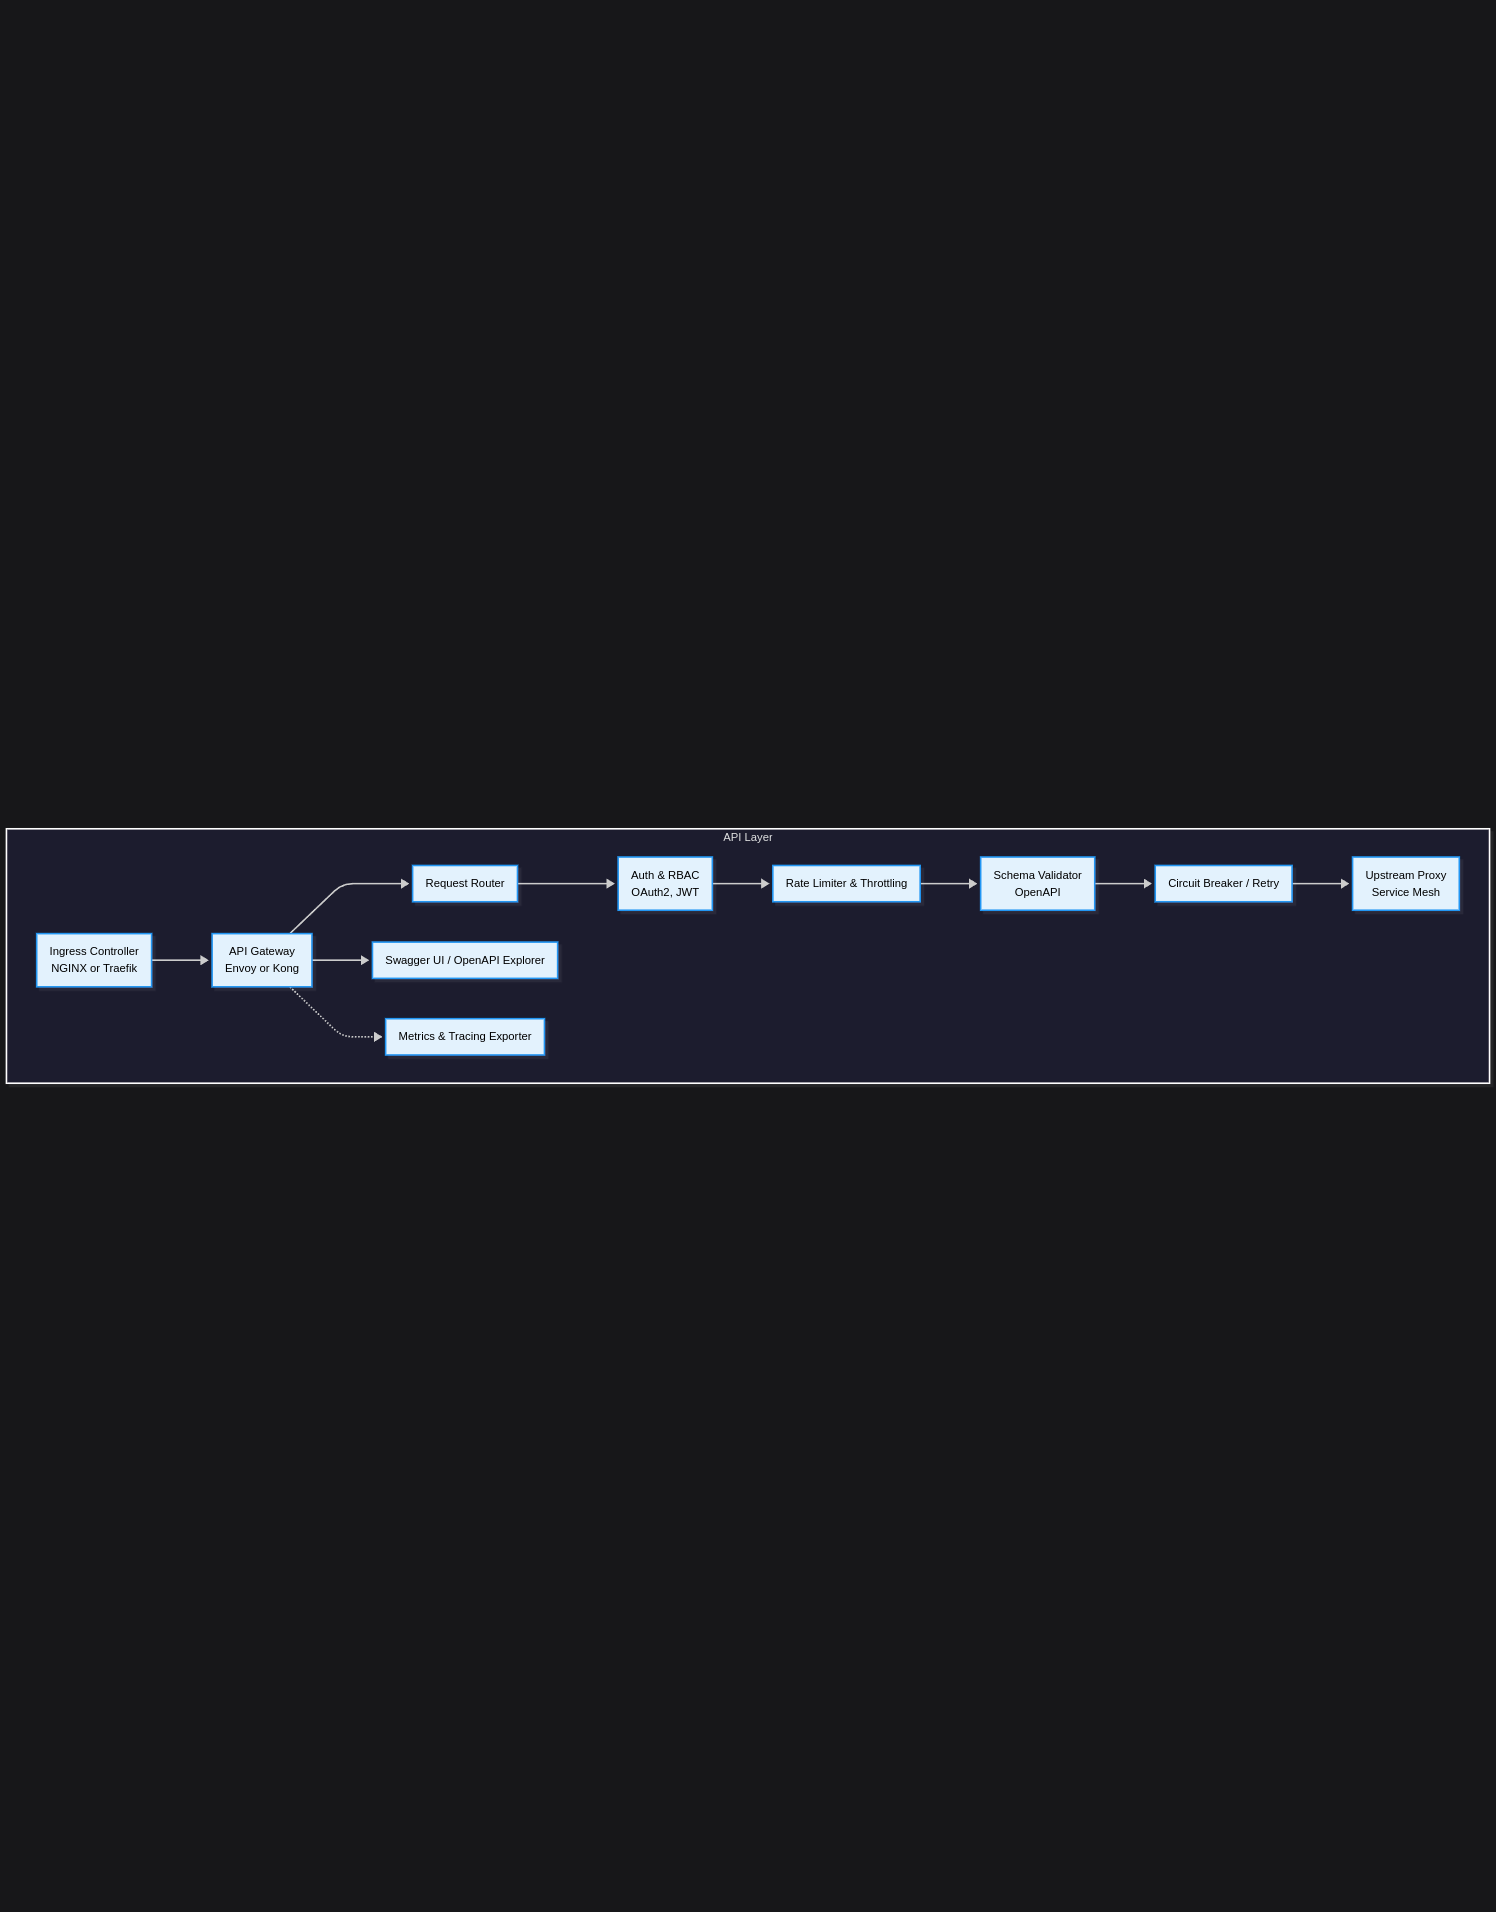
\includegraphics[width=0.5\textwidth]{core/layout.png} % Adjusted the scale of the image to 0.5
    \caption{System Architecture Overview}
  \end{figure}
\end{frame}

% \begin{frame}
%   \frametitle{Workflow}
%   \begin{figure}
%     \centering
%     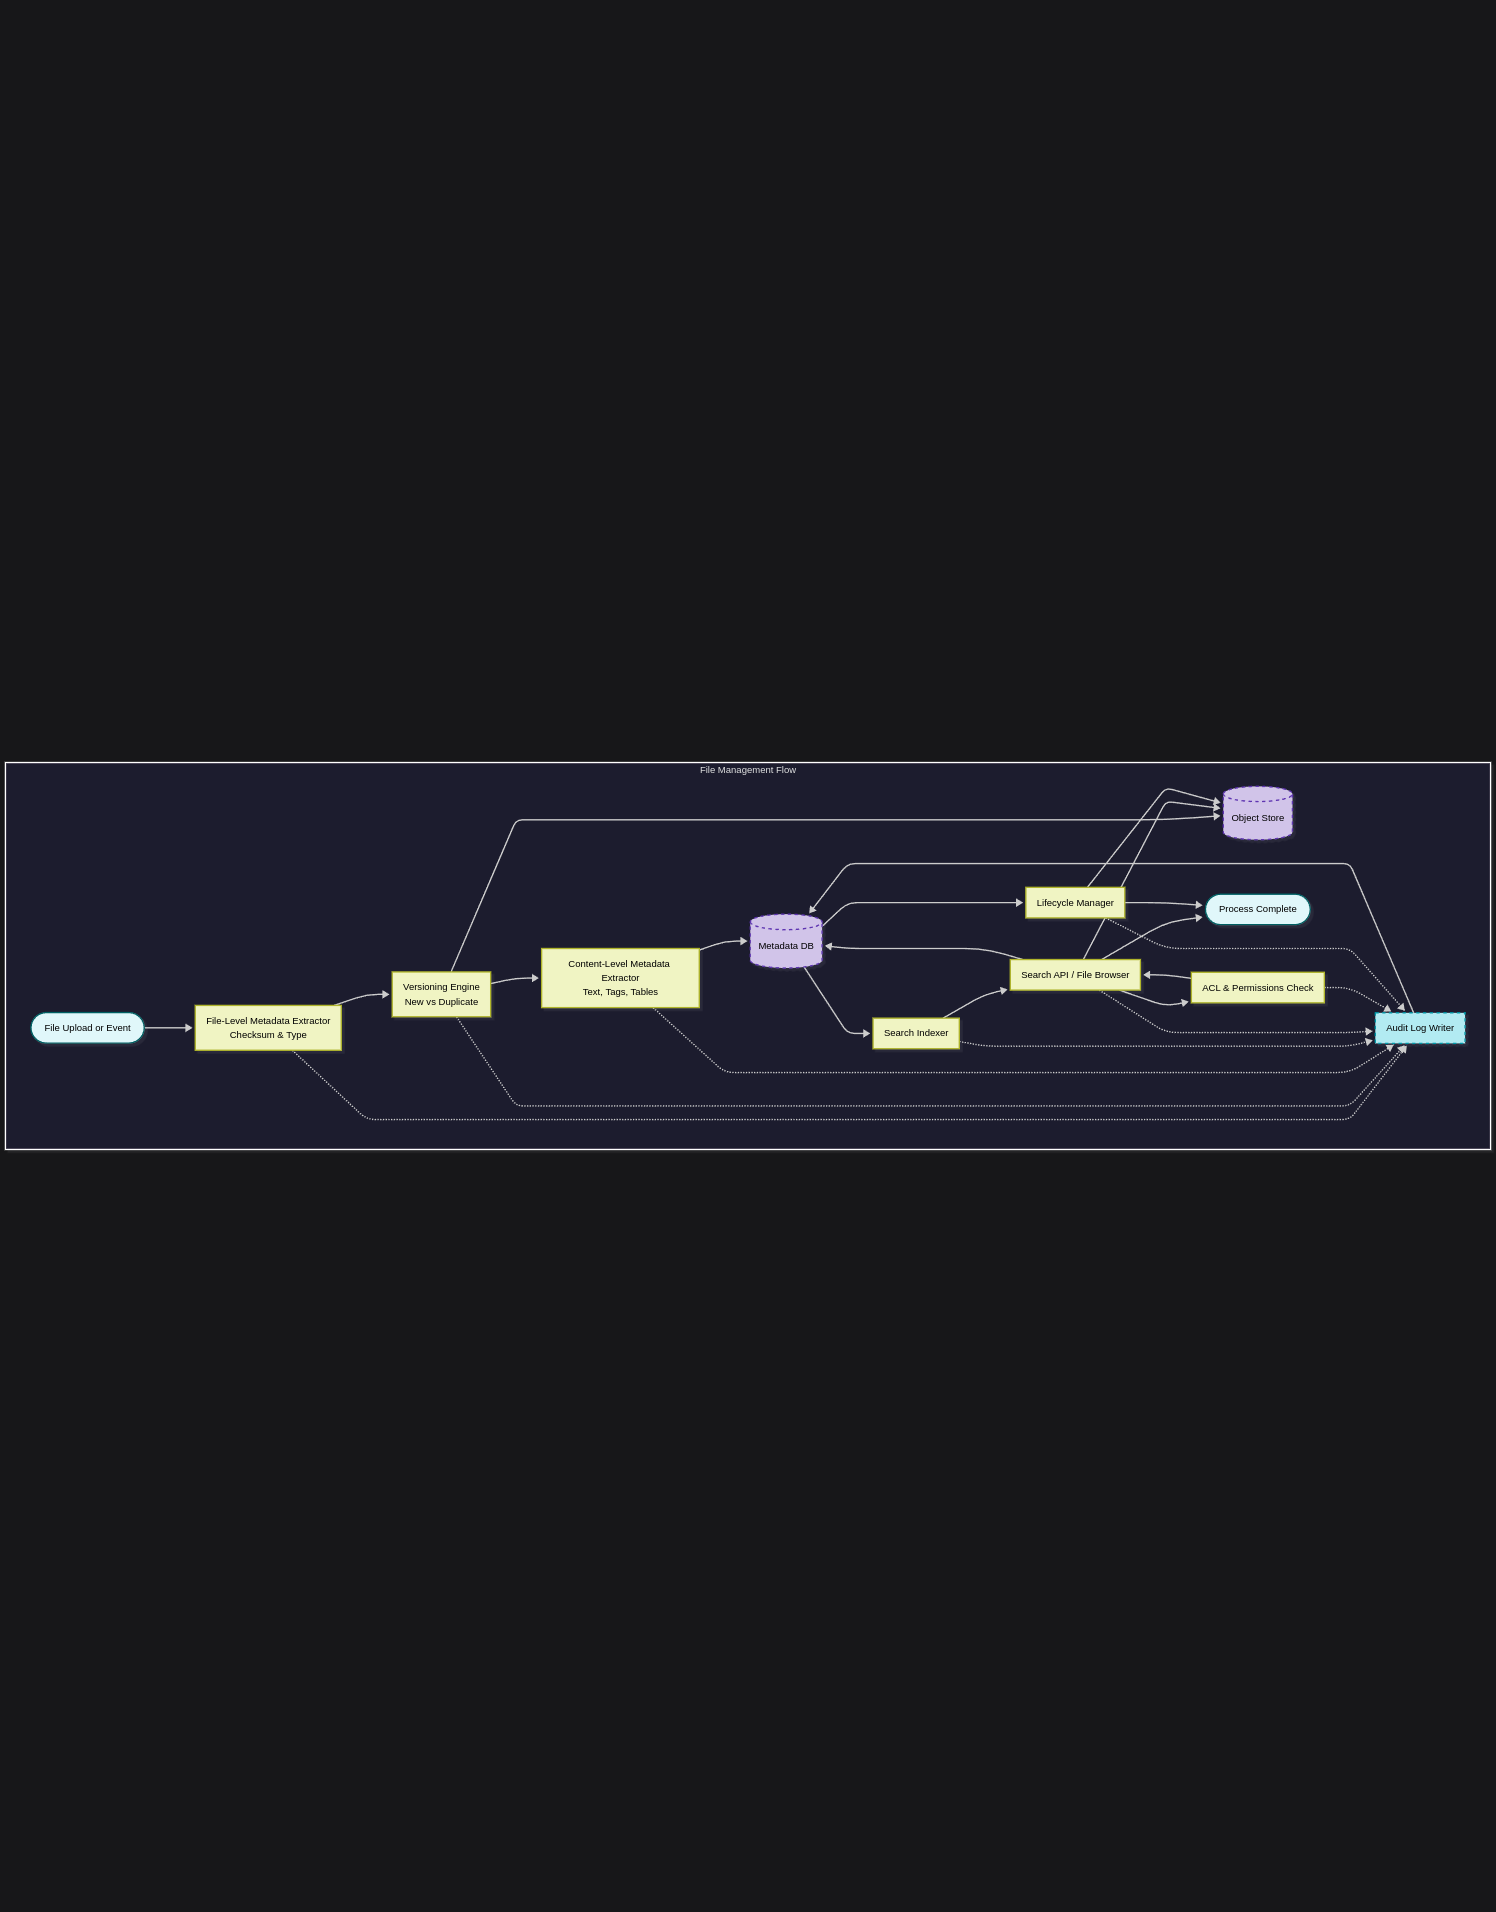
\includegraphics[width=0.8\textwidth]{core/flow.png} % Adjusted the scale of the image to 0.5
%     \caption{System Architecture Overview}
%   \end{figure}
% \end{frame}

% \begin{frame}
%   \frametitle{Sequence Flow}
%   \begin{figure}
%     \centering
%     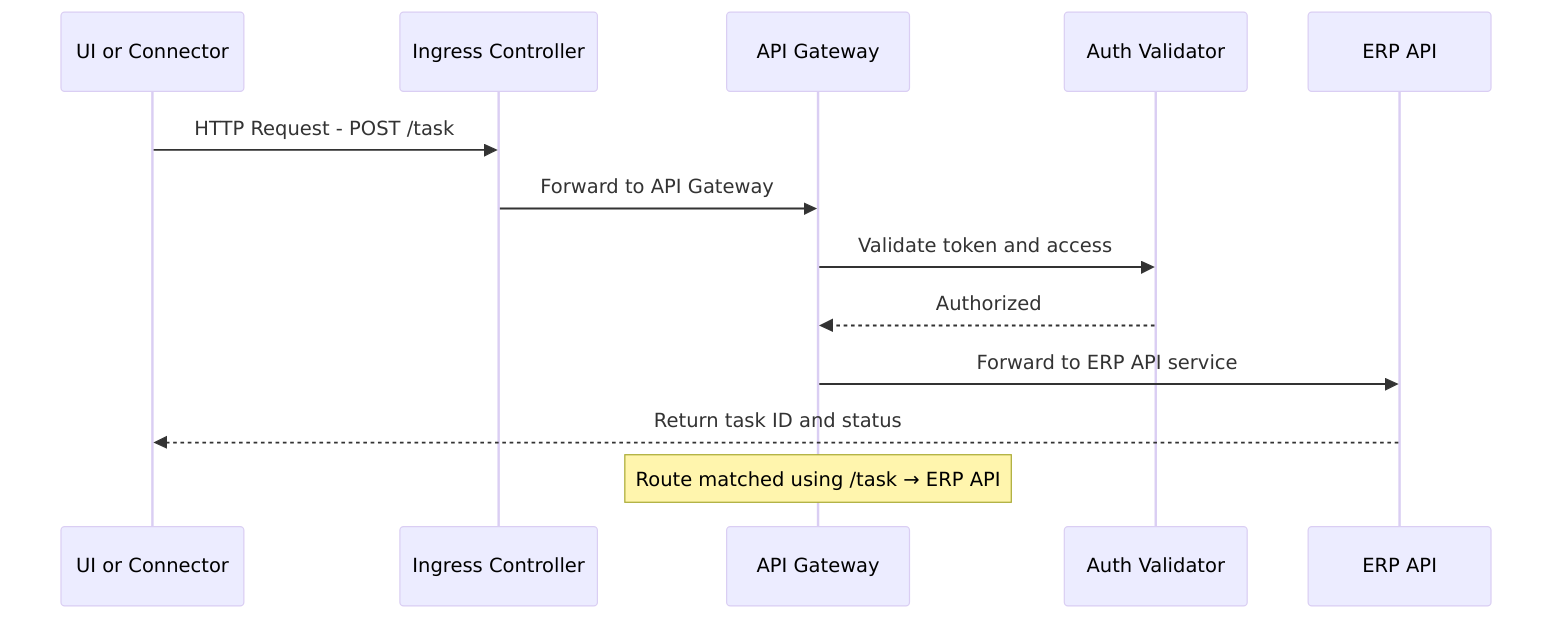
\includegraphics[width=0.8\textwidth]{core/sequence.pdf} % Adjusted the scale of the image to 0.5
%     \caption{System Architecture Overview}
%   \end{figure}
% \end{frame}

\begin{frame}
  \frametitle{Layer Functionalities - Part 1}
  \begin{itemize}
    \item \textbf{UI Layer}: Provides the user interface for document upload, agent triggering, task management, version review, change history, and analytics dashboards. Interfaces with API layer for all interactions.This layer contains an integration of chat assitant for user interaction.
    \item \textbf{API Layer}: Acts as the central access point via ingress and API gateway. Handles routing, authentication, rate limiting, versioned API groups (auth, agent, document, ETL, ERP, summary, compliance).
    \item \textbf{ERP Task Engine Layer}: Manages projects, tasks, workflows, approvals, assignments. Acts as the orchestrator connecting ETL, AI, and document systems with user workflows and audit logs.
    \item \item \textbf{AI Agent Layer}: Executes intelligent agents for document generation, compliance review, email understanding, P\&ID parsing, semantic diffing, enquiry processing, and task summaries.
    \item \textbf{ETL \& Digitisation Layer}: Ingests and watches file systems and document uploads. Computes checksums, extracts metadata, invokes AI-based content extraction, and stores structured outputs.
  \end{itemize}
\end{frame}



% System Architecture - Part 2
\begin{frame}
  \frametitle{Layer Functionalities}
  \begin{itemize}
    \item \textbf{Document System Layer}: Manages file uploads, versioning, semantic diffing, review flows, and links documents to tasks. Interfaces with storage and audit layers.
    \item \textbf{AI Agent Layer}: Executes intelligent agents for document generation, compliance review, email understanding, P\&ID parsing, semantic diffing, enquiry processing, and task summaries.
    \item \textbf{ETL \& Digitisation Layer}: Ingests and watches file systems and document uploads. Computes checksums, extracts metadata, invokes AI-based content extraction, and stores structured outputs.
    \item \textbf{Document System Layer}: Manages file uploads, versioning, semantic diffing, review flows, and links documents to tasks. Interfaces with storage and audit layers.
    \item \textbf{Storage Layer}: Handles object storage (MinIO/S3), metadata (MongoDB/Postgres), embeddings (vector DB), audit trails (TimescaleDB), and raw file lifecycle APIs.
  \end{itemize}
\end{frame}

% \begin{frame}
%   \frametitle{Layer Functionalities}
%   \begin{itemize}
%     \item \textbf{Observability Layer}: Provides monitoring, alerting, and logging for all components. Integrates with Grafana, Prometheus, and ELK stack for observability.
%     \item \textbf{Infra Layer}: Manages Kubernetes cluster, CI/CD pipelines, Helm charts, and Terraform scripts for infrastructure as code.
  
%   \end{itemize}
% \end{frame}


